\section{Musical Preliminaries}
\label{sec:music}

\paragraph{Pitches}
A \emph{pitch} is a value denoting how high or low a sound is.
In our implementation, pitches have type \texttt{Pitch} and take the
form \texttt{name octave}, where \texttt{name} is a name ranging
over \texttt{c}, \texttt{d}, \texttt{e}, etc. and \texttt{octave} is a
natural number denoting which octave the pitch belongs to.
For instance, the middle C is represented as \texttt{c 5}.

% \begin{alltt}
% data Pitch : Set where
%   pitch : \(\mathbb{N}\) \(\rightarrow\) Pitch

% data Octave : Set where
%   octave : \(\mathbb{N}\) \(\rightarrow\) Octave

% PitchOctave : Set
% PitchOctave = Fin 12 \(\times\) Octave
% \end{alltt}

\paragraph{Duration}
\emph{Duration} denotes an unspecified unit of time during which a
sound or silence lasts.
In our implementation, duration (of type \texttt{Duration} is simply
a natural number, denoting the relative length within a bar (such as
whole and half).
When the music is played at a specific tempo, the number is 
multiplied by a velocity and turned into an absolute length.

% \begin{alltt}
% data Duration : Set where
%   duration : \(\mathbb{N}\) \(\rightarrow\) Duration
% \end{alltt}

\paragraph{Notes}
Combining pitches and duration gives us \emph{notes}.
In our implementation, we represent notes as a datatype \texttt{Note}
with two constructors: \texttt{tone} for notes with sound and
\texttt{rest} for those without.

% \begin{alltt}
% data Note : Set where
%   tone : Duration \(\rightarrow\) Pitch \(\rightarrow\) Note
%   rest : Duration         \(\rightarrow\) Note
% \end{alltt}

\paragraph{Intervals}

\emph{Intervals} are a concept denoting the difference in pitch
between two notes.
There are 13 kinds of interval within an octave, and these intervals
can be classified from several different perspectives: (i) major or
minor; (ii) consonant or dissonant; and (iii) perfect or imperfect.
We define intervals as a datatype \texttt{Interval}, where each
constructor represents one of the 13 intervals.

\begin{figure}[h]
  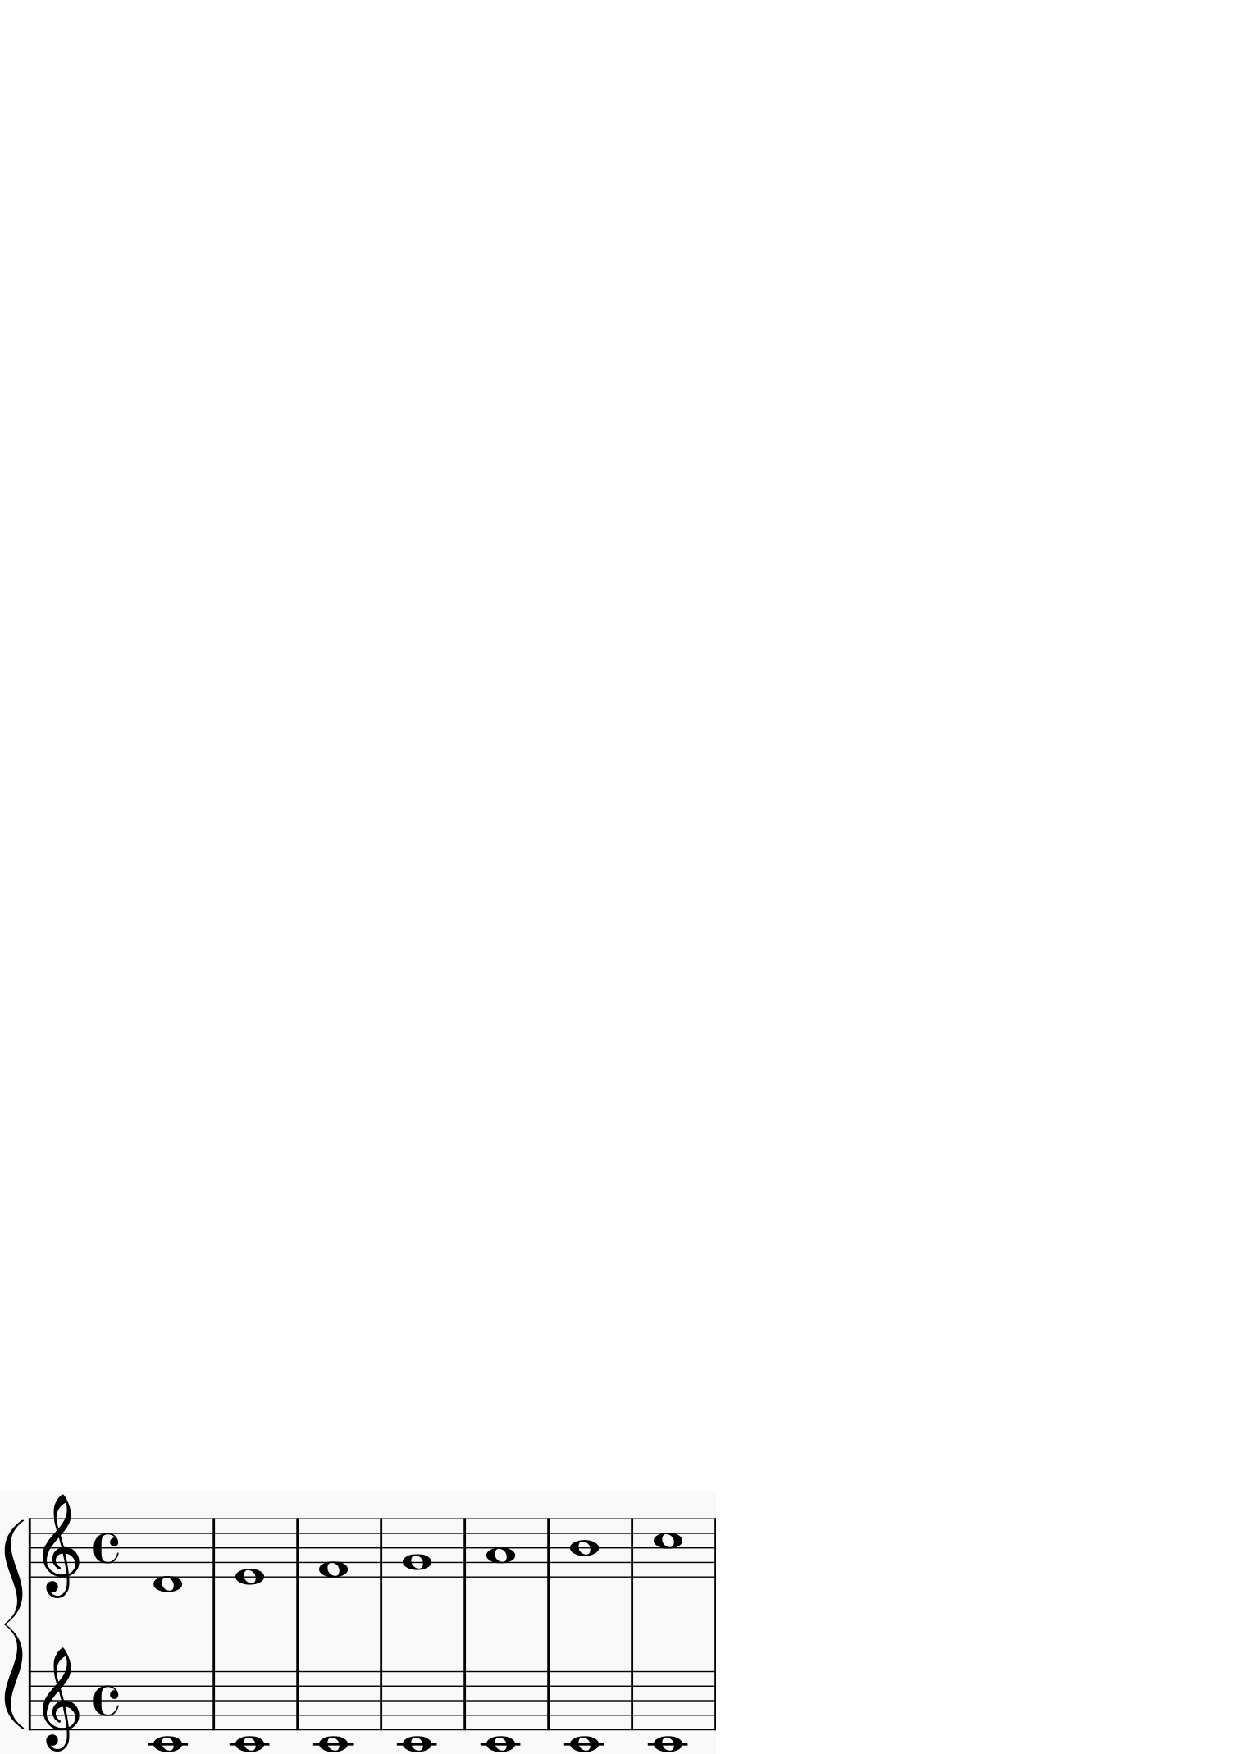
\includegraphics[width=12cm]{fig/interval.png} \\
  \begin{flushleft}
    \begin{footnotesize}
      \hspace{1.45cm} \texttt{per1 \hspace{0.5mm} min2  \hspace{2.5mm}
        maj2 \hspace{1.2mm} min3 \hspace{0.5mm} maj3 \ per4
        \hspace{1mm}aug4
        \hspace{0.5mm}  per5\hspace{1.2mm}  min6\hspace{1.6mm} maj6
        \hspace{1.6mm}min7\hspace{1.2mm} maj7\hspace{1.2mm} per8} \\
      consonant? \hspace{1.5mm} yes \hspace{4.2mm} no \hspace{6.5mm}  no
      \hspace{4.7mm} yes \hspace{3.8mm}  yes \hspace{3.7mm} no \hspace{3.5mm}
      no \hspace{4.3mm} yes \hspace{3.8mm} yes \hspace{3.2mm} yes
      \hspace{3.7mm} no \hspace{4mm} no \hspace{3.8mm} yes
    \end{footnotesize}
  \end{flushleft}
\end{figure}